%!TEX root = ../../book_ML.tex
\chapter{Triển khai chương trình và đánh giá hiệu suất}
\label{cha:chap3}
% \index{principal component analysis}
% \index{PCA -- \textit{xem} principle component analysis}
% \index{PCA}

% \index{phân tích thành phần chính -- principle component analysis}
% \index{principle component analysis -- phân tích thành phần chính}
% \index{PCA}
\section{Triển khai chương trình}
Về cơ bản để triển khai một bộ mã hóa tự động cho bài toán nén
có các bước chính sau:
\begin{itemize}[leftmargin=1.5cm]
    \item Thiết kế các lớp mạng
    \item Lựa chọn hàm đánh giá mất mát
    \item Lựa chọn thuật toán tối ưu
    \item Huấn luyện mô hình với tập dữ liệu cần nén
    \item Thực hiện nén, giải nén
\end{itemize}

Hoạt động nén được chia thành 2 quy trình:
\begin{itemize}[leftmargin=1.5cm]
    \item Huấn luyện mô hình (đại diện thao tác nén)
    \item Thực hiện nén, giải nén tập dữ liệu đã huấn luyện
\end{itemize}

\subsection{Thiết kế các lớp mạng}

Kết cấu của mạng này được thiết kế với 50 lớp chia thành 2 phần,
với các lớp tính chập đan xen lớp kích hoạt

\begin{figure}
    \begin{subfigure}{0.8\textwidth}
        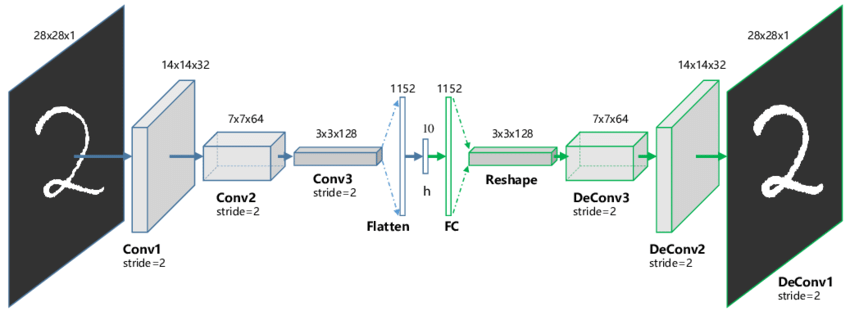
\includegraphics[width=1.\linewidth]{Chapters/items/networks.jpg}

        \label{fig: net1}
    \end{subfigure}
    \caption{Mô tả mô hình bộ mã hóa tự động đơn giản.}
\end{figure}

Thống kê số lượng tham số trong mạng, tương đương với số lượng các phép tính thực hiện
khi mỗi ảnh được truyền qua mạng.




\subsection{Lựa chọn thuật toán tối ưu}

Các thuật toán tối ưu trong học máy đã phát triển mạnh mẽ từ lâu và đã đạt đến mức hoàn thiện.
Hiện nay có một số thuật toán tối ưu nổi bật như sau :
\begin{itemize}[leftmargin=1.5cm]
    \item Adam \cite{Adadelta} là một trong những trình tối ưu hóa phổ biến nhất còn được gọi là Ước tính thời điểm thích ứng, nó kết hợp các thuộc tính tốt của Adadelta và trình tối ưu hóa RMSprop thành một và do đó có xu hướng làm tốt hơn cho hầu hết các vấn đề.
    \item Adagrad \cite{Adagrad} (viết tắt của adaptive gradient) xử phạt tốc độ học tập đối với các tham số được cập nhật thường xuyên, thay vào đó, nó cung cấp tốc độ học tập nhiều hơn cho các tham số thưa thớt, các tham số không được cập nhật thường xuyên.
    \item Stochastic gradient descent \cite{svd} là cực kỳ cơ bản và hiếm khi được sử dụng bây giờ. Một vấn đề là với tỷ lệ học tập trên toàn thế giới liên quan đến một tương đương. Do đó, nó không hoạt động tốt khi các thông số ở nhiều thang đo vì tốc độ học cà phê sẽ làm cho quá trình đào tạo chậm lại trong khi tốc độ học tập quá lớn có thể gây ra dao động. Ngoài ra, dốc Stochastic đi xuống thường gặp khó khăn khi thoát khỏi các điểm yên ngựa. Adagrad, Adadelta, RMSprop và ADAM thường xử lý các điểm yên ngựa tốt hơn. SGD với xung lượng đưa ra một số tốc độ tối ưu hóa và cũng giúp thoát cực tiểu cục bộ tốt hơn.
\end{itemize}

Nhưng sau khi thực hiện những thử nghiệm nhỏ đơn giản, thì chúng em quyết định
lựa chọn thuật toán tối ưu Adam, là thuật toán đạt độ mất mát thấp và tốc độ hội tụ
để hướng đến nghiệm tối ưu của bài toán tốt.


\subsection{Lựa chọn hàm đánh giá mất mát}

Cũng giông như các thuật toán tối ưu, các hàm đánh giá mất mát cũng đã được phát triển và
hoàn thiện từ lâu, có một số hàm đánh giá nổi bật như sau:
\begin{itemize}
    \item Cross Entropy: Suy hao chéo entropy hay còn gọi là mất log, đo lường hiệu suất của mô hình phân loại có đầu ra là giá
          trị xác suất từ 0 đến 1. Mất entropy chéo tăng lên khi xác suất dự đoán khác với nhãn thực tế. Vì vậy,
          dự đoán xác suất bằng 0,12 khi nhãn quan sát thực tế là 1 sẽ không tốt và dẫn đến giá trị tổn thất cao.
          Một mô hình hoàn hảo sẽ có lỗ nhật ký bằng 0.
    \item Hinge - Thường dùng trong các bài toán phân loại
    \item Huber - Thường được sử dụng để hồi quy. Nó ít nhạy cảm hơn với các ngoại lệ so với MSE vì nó coi lỗi là hình vuông chỉ trong một khoảng thời gian.
    \item MAE, MSE - Là phép tính chuẩn 1, chuẩn 2 thường xuất hiện rất nhiều trong các bài
          toán học máy vì tính đơn giản mà hiệu quả mà nó mang lại.
\end{itemize}

Vì đây là bài toán so sánh độ tương đồng giữa ảnh nên chúng em lựa chọn MSE làm phương pháp đánh giá mất mát cho mô hình


\subsection{Huấn luyện mô hình với tập dữ liệu cần nén}
\subsubsection{Tập dữ liệu sử dụng}

Ở đây, để tăng tính ngẫu nhiên chúng em sử dụng 1 tập dữ liệu ảnh màu với các
kích thước giống nhau (768x1280) được cung cấp từ một thư viện lấy các ảnh ngẫu
nhiên từ các video trên nền tảng Youtube. Với số lượng là 2286 ảnh chất
lượng cao, tổng dung lượng lưa trữ là 6.3 GB

\begin{figure}
    \begin{subfigure}{0.6\textwidth}
        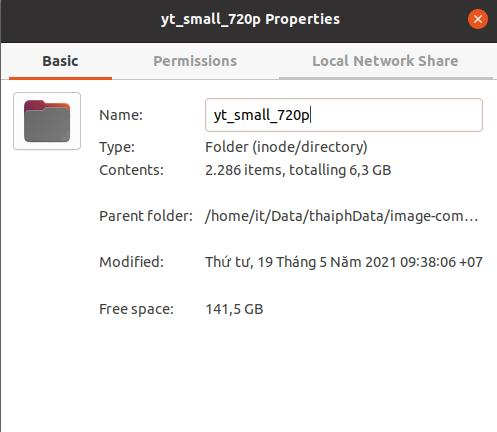
\includegraphics[width=1.\linewidth]{Chapters/items/data.jpg}

        \label{fig: data}
    \end{subfigure}
    \caption{Tập dữ liệu sử dụng}
\end{figure}

\subsubsection{Các tham số huấn luyện mô hình}
Khi huấn luyện một mô hình mạng nơ-ron nhận tạo điển hình có
các tham số như là : số kỷ nguyên (epoch), Kích thước lô (batch size),
số lân lặp lại (Iterations)

Đối với mô hình này chúng ta phải lựa chọn thêm 1 số tham số giống như
số luồng (thread), tỷ lệ học (learning rate) để mô hình trở lên linh hoạt hơn

\newpage
Với GPU Tesla T4 16GB, được cung cấp bởi Google Colab và dữ liệu
2286 ảnh chúng em lựa chọn các tham số kích thước lô là 16, số kỷ nguyên là 3,
tỉ lệ học tập là 0,0001, số luồng chạy là 5

\begin{figure}
    \begin{subfigure}{0.7\textwidth}
        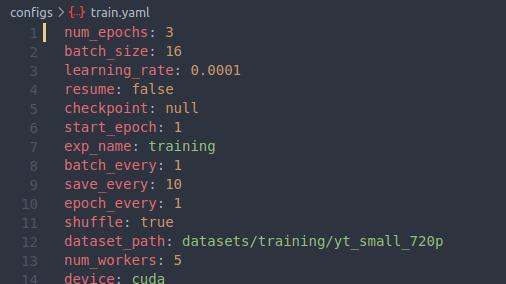
\includegraphics[width=1.\linewidth]{Chapters/items/pram.jpg}

        \label{fig: param}
    \end{subfigure}
    \caption{Các tham số được lựa chọn}
\end{figure}

\subsubsection{Quá trình huấn luyện mô hình}

\begin{figure}
    \begin{subfigure}{1.\textwidth}
        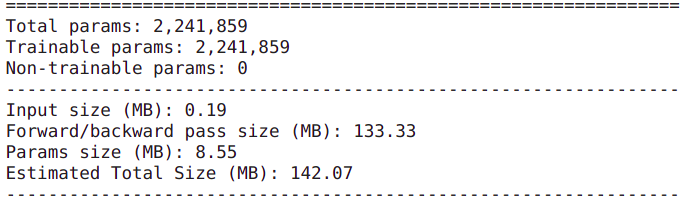
\includegraphics[width=1.\linewidth]{Chapters/items/model.png}
        \label{fig: model}
    \end{subfigure}
    \caption{Thông tin tổng quan của mạng}
\end{figure}

Mạng nơ-ron có tổng số tham số khoảng 2 triệu tham số với 50 lớp mạng chủ yếu
là các lớp tích chập, phi tuyến.



Tổng thời gian khi huấn luyện mô hình là khoảng 30 phút, điều này
đại diện cho thời gian nén mặc dù vẫn chưa thực sự tối ưu về mặt
thời gian, nhưng chúng em tin rằng khi phần cứng mạnh mẽ hơn thì
thời gian nén cũng sẽ giảm đi đáng kể.

\begin{figure}
    \begin{subfigure}{0.8\textwidth}
        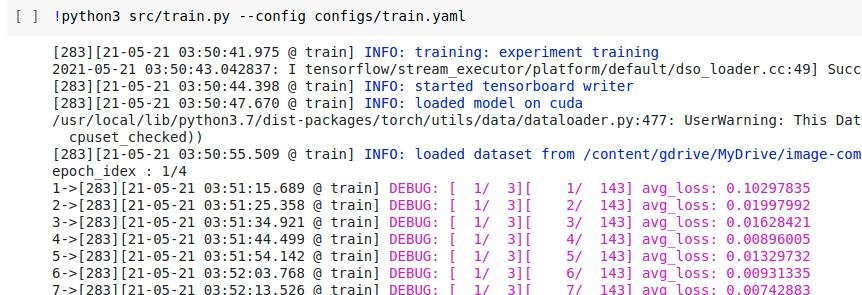
\includegraphics[width=1.\linewidth]{Chapters/items/colab1.jpg}

        \label{fig: colab1}
    \end{subfigure}
    \caption{Khởi đầu quá trình huấn luyện}
\end{figure}

\newpage
Có thể thấy rằng tham số avg-loss (đánh giá sứ mất mát) từ lúc
bắt đầu huấn luyện cho đến khi kết thúc đã giảm đi rất đáng kể
cho thấy tính đúng đắn của mô hình, dự báo rằng mô hình sẽ đạt kết
quả thử nghiệm tốt.

\begin{figure}
    \begin{subfigure}{0.8\textwidth}
        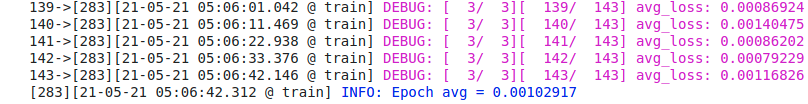
\includegraphics[width=1.\linewidth]{Chapters/items/colab2.jpg}

        \label{fig: colab2}
    \end{subfigure}
    \caption{Kết thúc quá trình huấn luyện}
\end{figure}

Mô hình hóa quá trình huấn luyện sử dụng tensorboard :
(Trục ngang là số lần lặp lại, trục đứng là đánh giá mất mát)

\begin{figure}
    \begin{subfigure}{0.8\textwidth}
        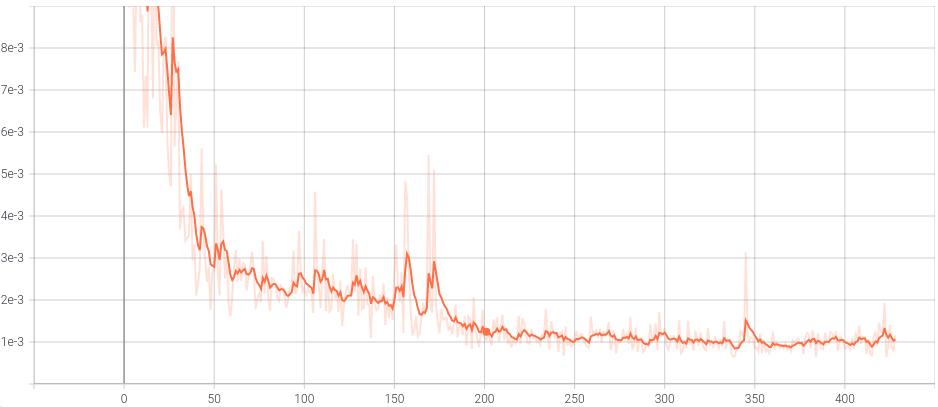
\includegraphics[width=1.\linewidth]{Chapters/items/visualizeTraining.jpg}

        \label{fig: visualize}
    \end{subfigure}
    \caption{Quá trình giảm của mất mát theo số lần lặp lại các lô}
\end{figure}

\subsection{Thực hiện nén, giải nén}


\begin{itemize}
    \item Đầu vào của chương trình nén là ảnh với các thông số 768x1280x3 (lần lượt là chiều rộng, chiều cao, số kênh màu)
    \item Sau khi ảnh đươc đưa vào bộ nén sẽ được nén thành dạng 6x10x32x32x32
    \item Khi đưa file nén vào bộ giải nén ảnh sẽ được khôi phục lại kích thước 768x1280x3
\end{itemize}

\subsubsection{Nén}
Vì mạng nơ-ron chỉ nhận những đầu vào có kích thước nhỏ nên ảnh đầu vào sẽ được chia
làm 60 phần bằng nhau tức kích thước ban đầu là 768x1280x3 sẽ được chia thành 60x128x128x3

Và 60 hình nhỏ này sẽ lần lượt chạy qua mạng và sẽ được lặp đi lặp lại một số lần
trong qúa trình học của mạng để tạo ra các khối được nén lại. Các khối này có kích thước
32*32*32.

\begin{figure}
    \begin{subfigure}{0.8\textwidth}
        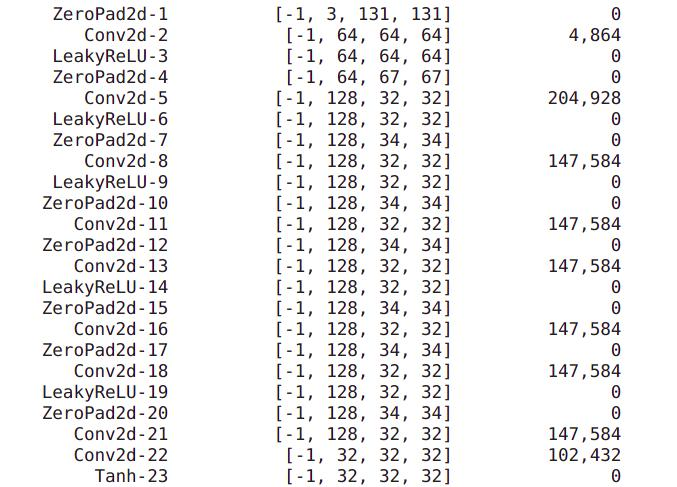
\includegraphics[width=1.\linewidth]{Chapters/items/encode.jpg}

        \label{fig: encode}
    \end{subfigure}
    \caption{Các lớp mạng tham gia vào quá trình nén}
\end{figure}

\subsubsection{Giải nén}

Khi các khối nén 32x32x32 đã được học xong thì chúng ta lưu nó lại như là thành phần chính
của file nén.

Một thành phần nữa không thể thiếu đó chính là các bộ trọng số đại diện cho
tri thức của mạng sau khi đã học nén và giải nén.

Khi thực hiện giải nén, chúng ta lại đưa file nén gồm nhiều các khối 32x32x32 vào mô hình giảm mã
lần lượt để mô hình có thể giải mã giống như những gì nó đã học được trong quá trình huấn luyện
để được các đầu ra mong muốn là các khối 128x128x3
. Và các khối này lại được sắp xếp để khôi phục ảnh với kích thước ban đầu 768x1280x3


\begin{figure}
    \begin{subfigure}{0.8\textwidth}
        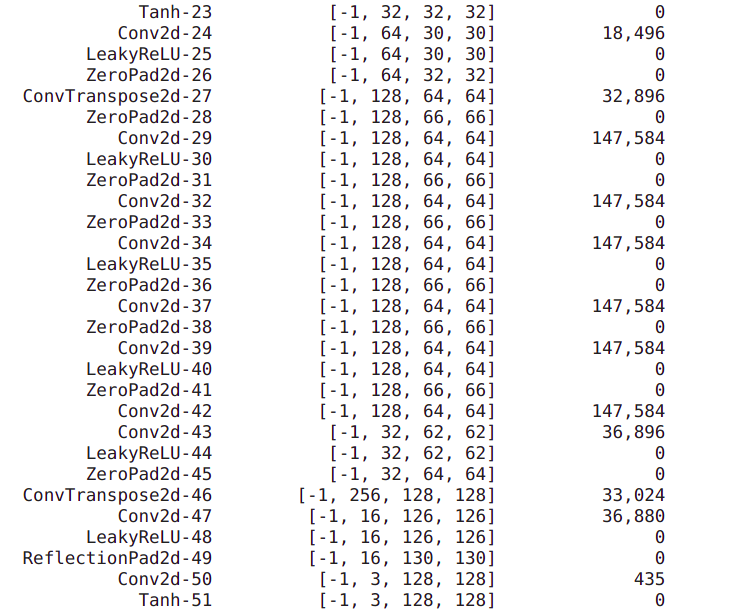
\includegraphics[width=1.\linewidth]{Chapters/items/decode.jpg}
        \label{fig: decode}
    \end{subfigure}
    \caption{Các lớp mạng tham gia vào quá trình giải nén}
\end{figure}


\newpage
\section{Đánh giá hiệu suất nén}

Sau khi thực hiện các quá trình nén và giải nén thì thu được kết quả như sau:

\begin{figure}
    \begin{subfigure}{1.\textwidth}
        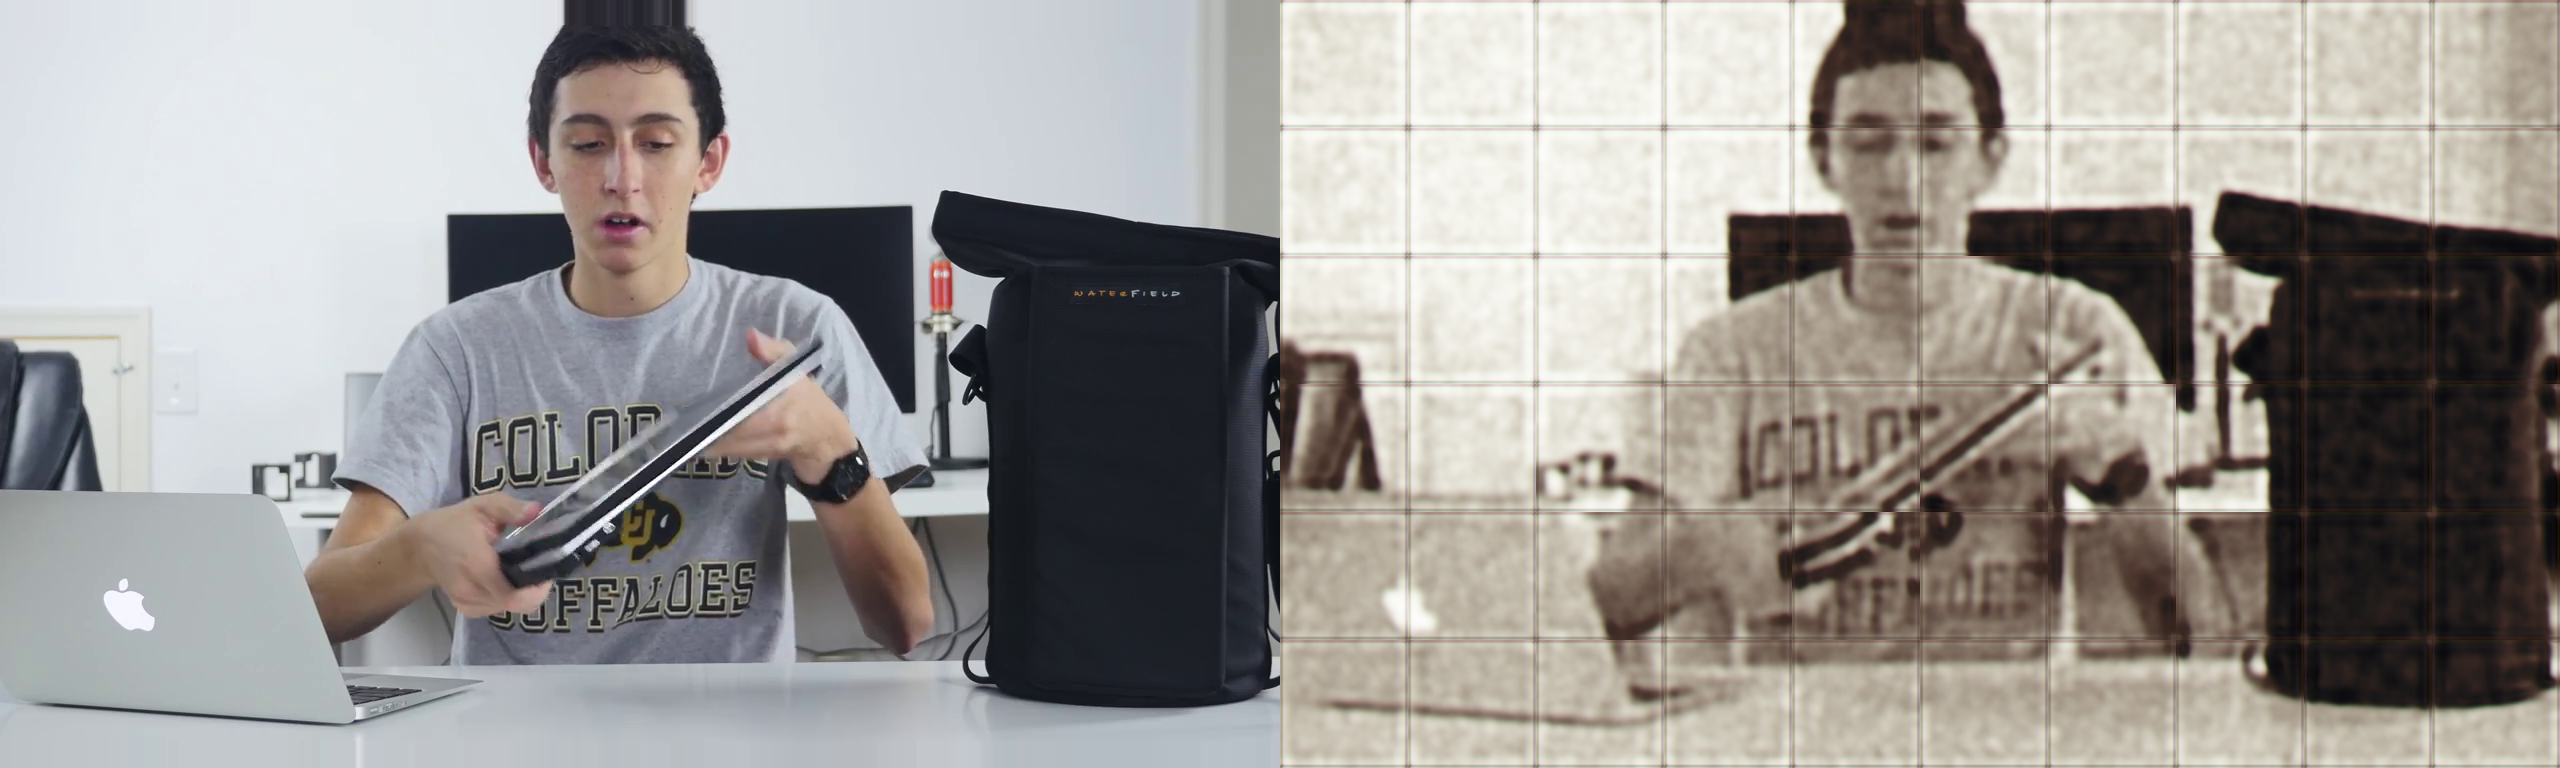
\includegraphics[width=1.\linewidth]{Chapters/items/1_10.png}
        \label{fig: 1epoch}
    \end{subfigure}
    \caption{Ảnh khi qua kỷ nguyên đầu tiên}
\end{figure}

\begin{figure}
    \begin{subfigure}{1.\textwidth}
        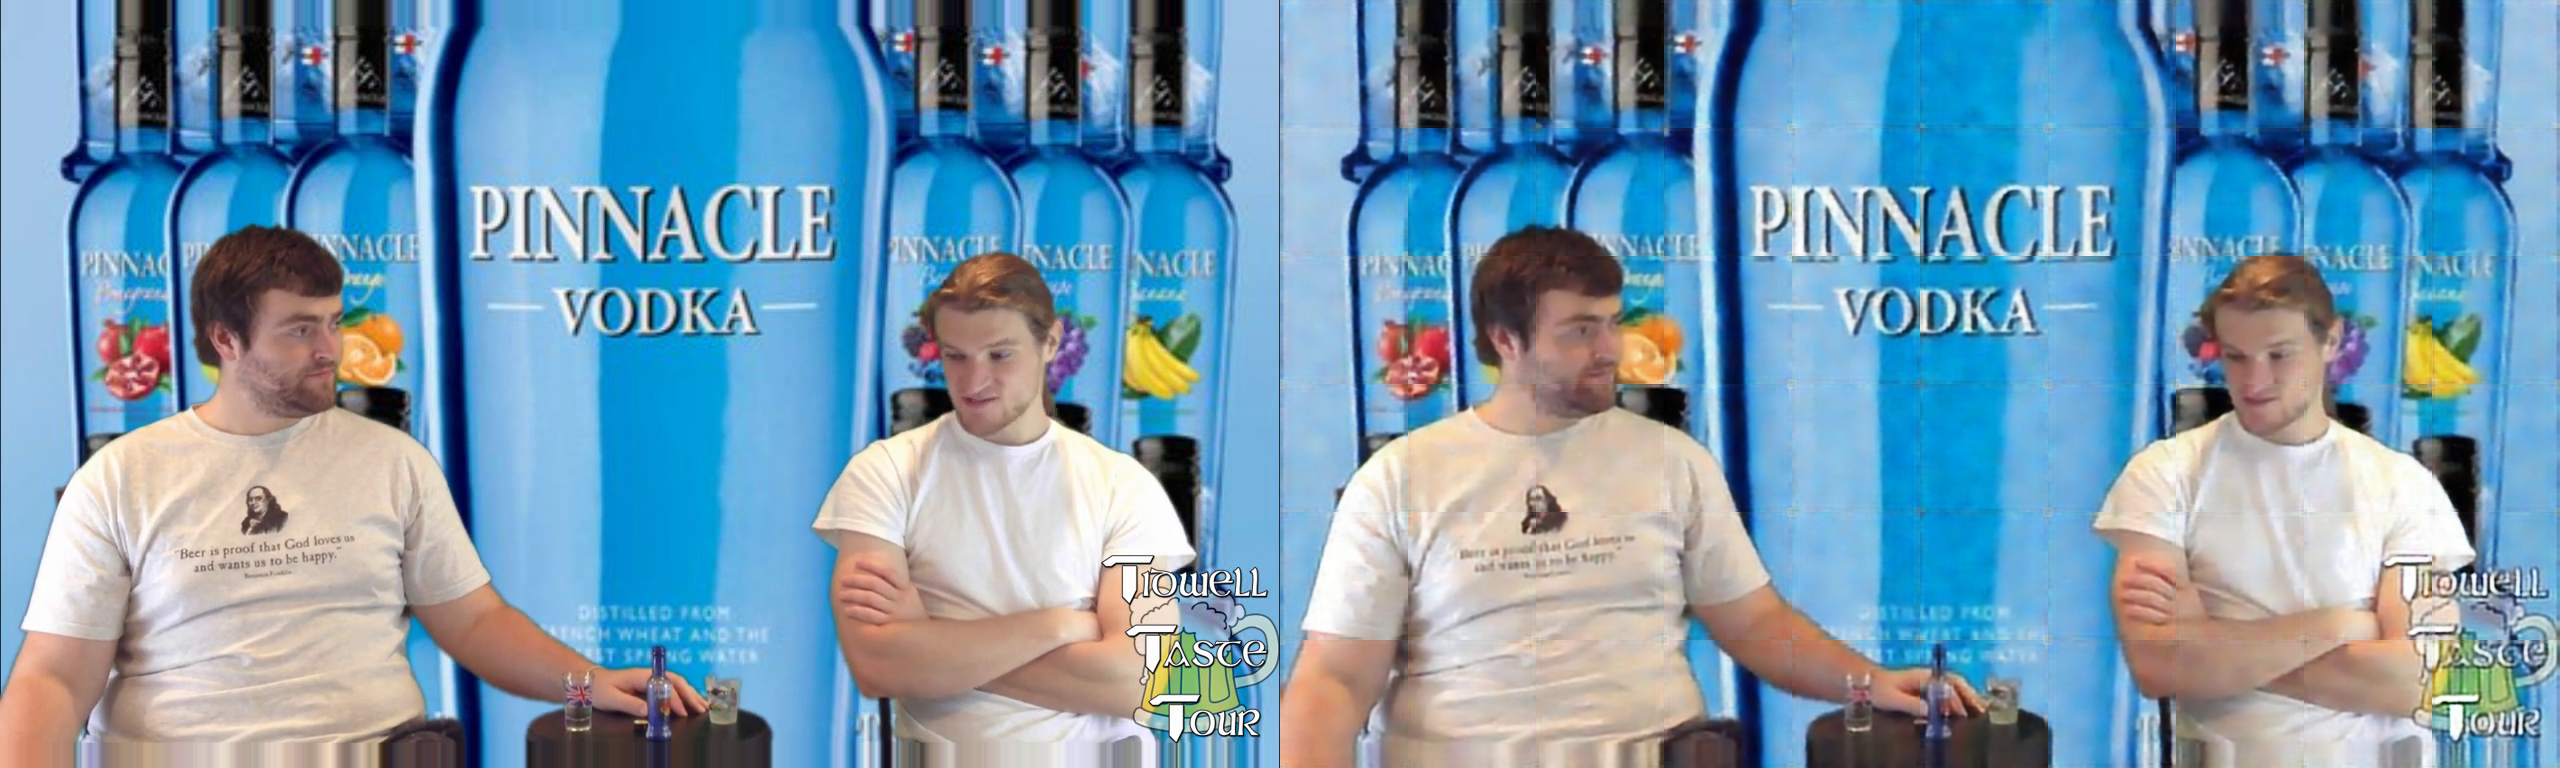
\includegraphics[width=1.\linewidth]{Chapters/items/3_30.png}
        \label{fig: 3_30epoch}
    \end{subfigure}
    \caption{Ảnh khi qua kỷ nguyên thứ 250}
\end{figure}

\begin{figure}
    \begin{subfigure}{1.\textwidth}
        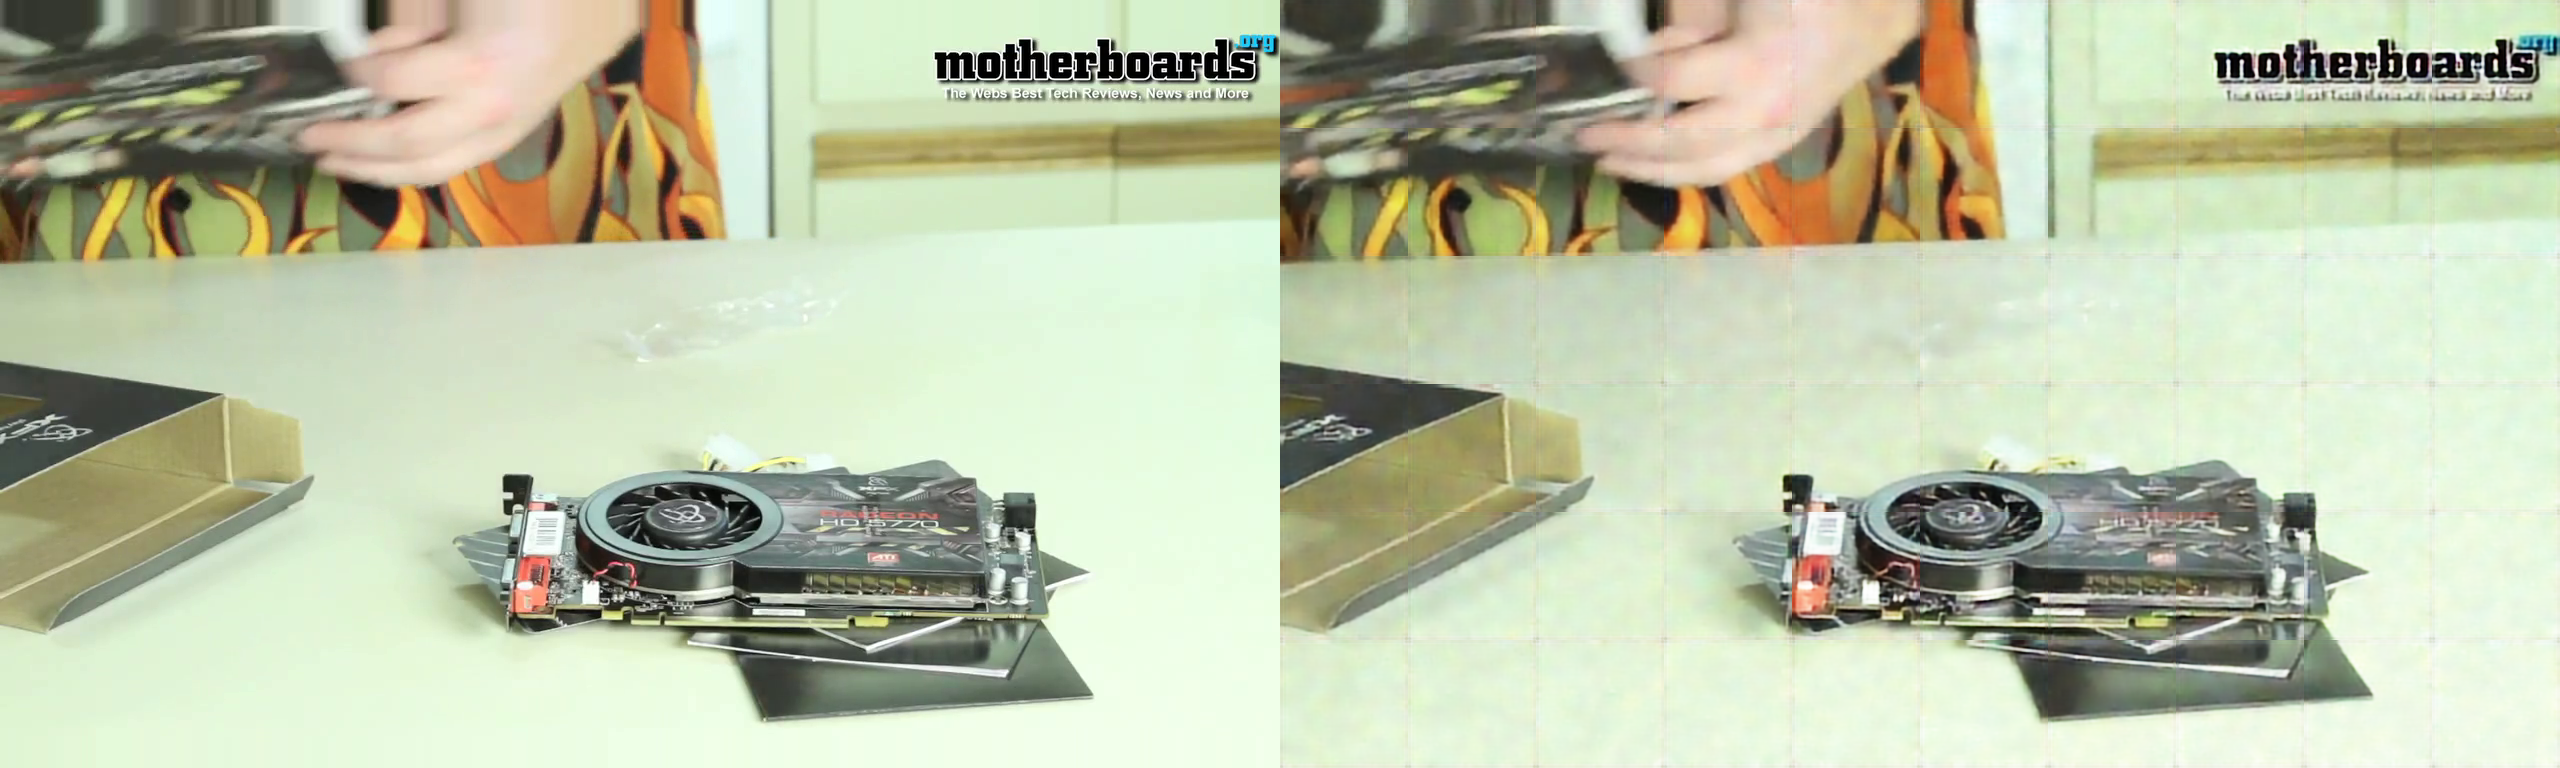
\includegraphics[width=1.\linewidth]{Chapters/items/3_100.png}
        \label{fig: 3_100epoch}
    \end{subfigure}
    \caption{Ảnh khi qua kỷ nguyên thứ 380}
\end{figure}

\begin{figure}
    \begin{subfigure}{1.\textwidth}
        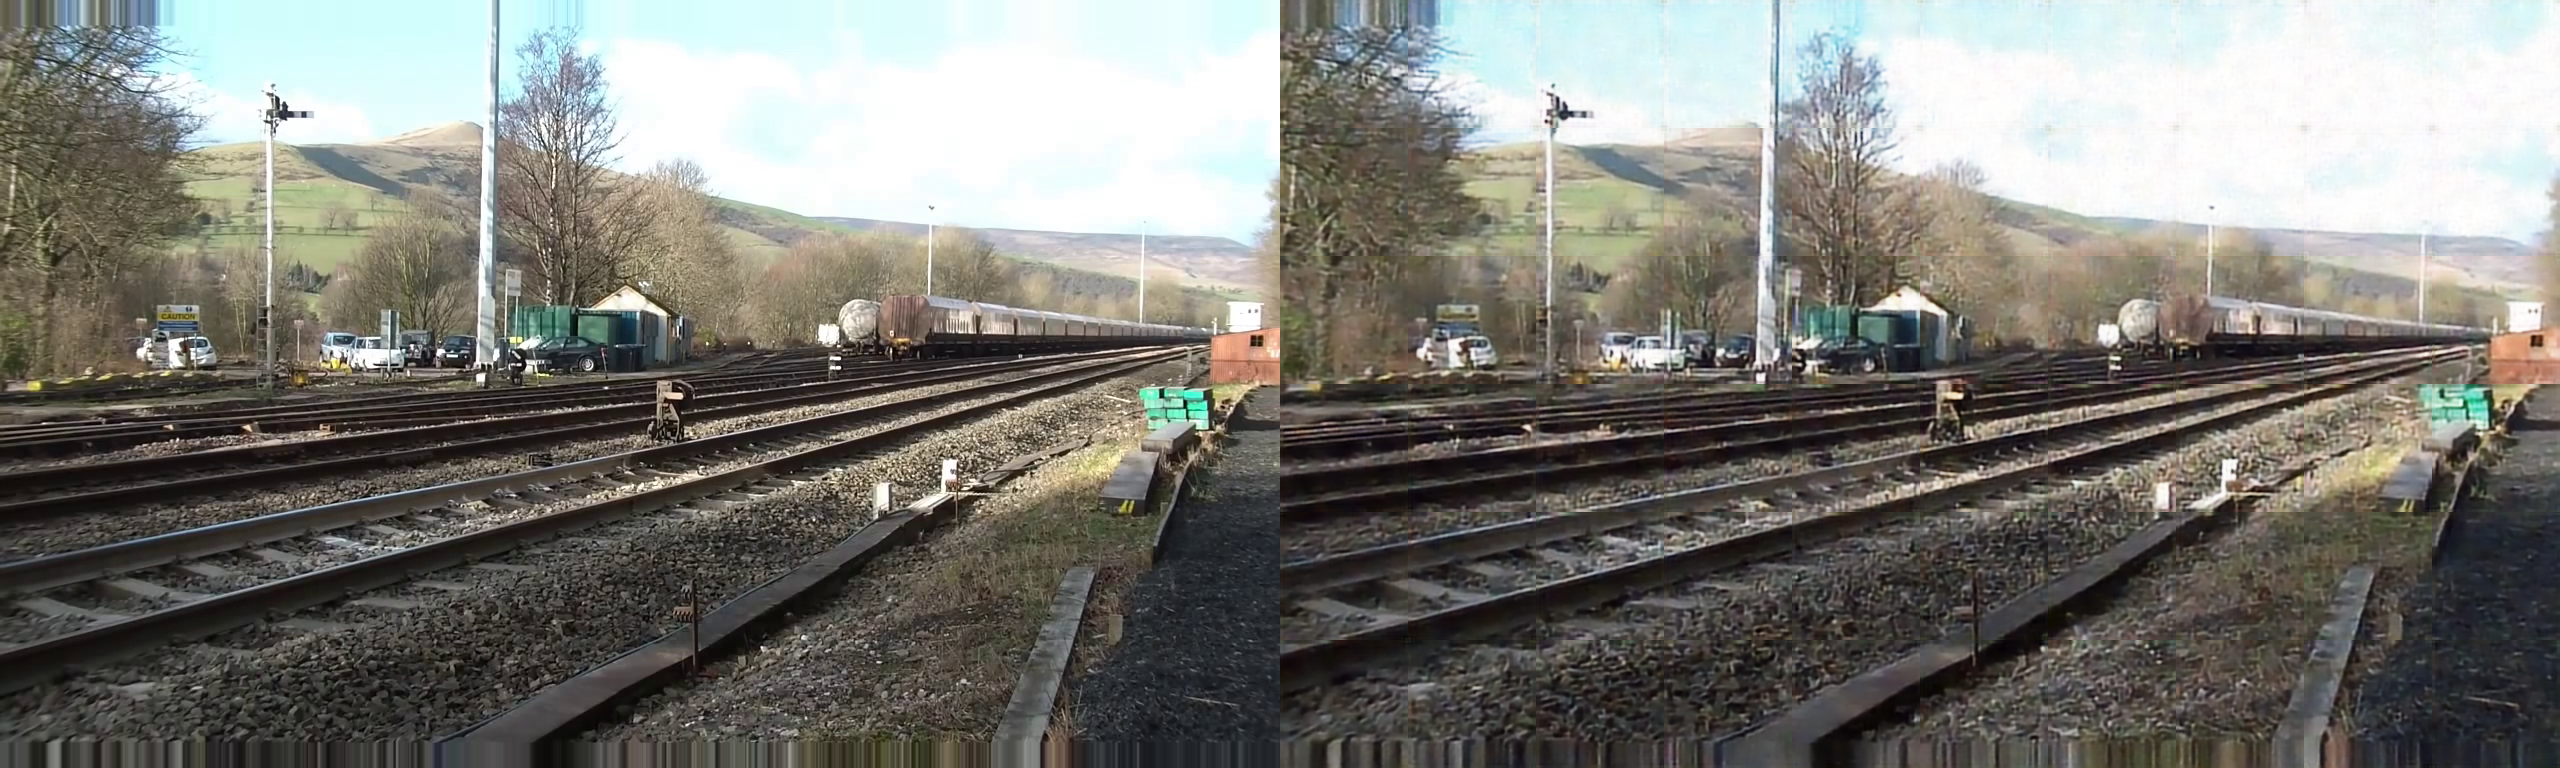
\includegraphics[width=1.\linewidth]{Chapters/items/3_140.png}
        \label{fig: 3_140epoch}
    \end{subfigure}
    \caption{Ảnh khi qua kỷ nguyên cuối cùng}
\end{figure}



